\documentclass[12pt,a4paper]{article}
\usepackage{cmap}
\usepackage{amsmath}
\usepackage{amsfonts}
\usepackage{mathtext}
\usepackage{titlesec}
\usepackage{float}
\usepackage{subcaption}
\usepackage{amssymb}
\usepackage{tikz}
\usetikzlibrary{positioning, arrows.meta, shapes.geometric}
\usepackage[utf8]{inputenc}
\usepackage[T2A]{fontenc}
\usepackage{wrapfig}
\usepackage[english, russian]{babel}
\usepackage[left=2cm,right=2cm,top=2cm,bottom=2cm]{geometry}
\usepackage{indentfirst}

\DeclareSymbolFont{T2Aletters}{T2A}{cmr}{m}{it}

%%% Работа с картинками
\usepackage{graphicx}  % Для вставки рисунков
\graphicspath{{imgs/}}  % папки с картинками

\usepackage{caption}
\captionsetup{labelsep=period, labelfont=bf}

\titleformat{\section}[block]
{\normalfont}{\thesection.}{0 cm}{}
\titleformat{\subsection}[block]
{\bfseries}{\thesubsection.}{0 cm}{}

\titlespacing{\section}{17pt}{14pt}{10pt}
\titlespacing{\subsection}{17pt}{14pt}{4pt}

\def \TITLE {Отчет о выполнении лабораторной работы №5}
\def \SUBTITLE {Определение числа Рейнольдса перехода к турбулентности в пограничном слое}
\def \AUTHOR {Выполнилb студентs группы Б03-405\\ Подшивалова Анастасия \\ Савельева Александра \\ Собкина Ксения\\ Тимохин Даниил\\ Трифонова Анна}
\def \DATE {16 февраля 2026 г.}

\begin{document}

\begin{titlepage}
	\centering
	\vspace{5cm}
	{\scshape\large Московский физико-технический институт \\
	(национальный исследовательский университет)}
	
	\vspace{4cm}
	{\LARGE \TITLE}
	
	\vspace{1cm}
	{\Huge\bf \SUBTITLE }
	
	\vspace{1cm}
	\vfill
	
\begin{flushright}
	{\LARGE \AUTHOR}
\end{flushright}
	

	\vfill

	\DATE
\end{titlepage}

\newpage

\fontsize{12}{14}\selectfont

\section{ Аннотация}



\section{ Теоретическая справка}


При обтекании твердого тела реальной жидкостью или газом вследствие вязкости возникает прилипание среды к поверхности. Скорость потока на стенке равна нулю и увеличивается по мере удаления от нее до скорости внешнего потока $U_\infty$. Тонкий слой жидкости у поверхности, в котором вязкость существенно влияет на течение, называется \textbf{пограничным слоем}.

Касательное напряжение в вязкой среде определяется законом Ньютона:
\begin{equation}
\tau = \mu \frac{dU}{dy}, \tag{1}
\end{equation}
где $\mu$ — коэффициент динамической вязкости.

Характер течения определяется безразмерным числом Рейнольдса
\begin{equation}
Re = \frac{\rho U L}{\mu}, \tag{2}
\end{equation}
которое характеризует отношение сил инерции к силам вязкости. Здесь $\rho$ — плотность среды, $U$ — характерная скорость, $L$ — характерный линейный размер.

Толщиной пограничного слоя $\delta$ считают расстояние от поверхности, на котором скорость достигает значения
\begin{equation}
U = 0.99 U_\infty. \tag{3}
\end{equation}

Для ламинарного пограничного слоя на плоской пластине
\begin{equation}
\frac{\delta}{x} = 5 \left( \frac{U_\infty x}{\nu} \right)^{-1/2}, \tag{4}
\end{equation}
а для турбулентного пограничного слоя
\begin{equation}
\frac{\delta}{x} = 0.37 \left( \frac{U_\infty x}{\nu} \right)^{-1/5}, \tag{5}
\end{equation}
где $\nu = \mu / \rho$ — кинематическая вязкость.

Важными интегральными характеристиками пограничного слоя являются толщина вытеснения и толщина потери импульса. Толщина вытеснения $\delta^*$ характеризует уменьшение расхода жидкости в пограничном слое из-за уменьшения скорости потока вблизи поверхности и определяется выражением
\begin{equation}
\delta^* = \int_0^\infty \left( 1 - \frac{U}{U_\infty} \right) dy. \tag{6}
\end{equation}
Физически она равна такому смещению границы потенциального потока.

Толщина потери импульса $\delta^{**}$ определяется как
\begin{equation}
\delta^{**} = \int_0^\infty \frac{U}{U_\infty} \left( 1 - \frac{U}{U_\infty} \right) dy. \tag{7}
\end{equation}

Для ламинарного пограничного слоя
\begin{equation}
\frac{\delta^{**}}{x} = 0.664 \left( \frac{U_\infty x}{\nu} \right)^{-1/2}, \tag{8}
\end{equation}
а для турбулентного
\begin{equation}
\frac{\delta^{**}}{x} = 0.036 \left( \frac{U_\infty x}{\nu} \right)^{-1/5}. \tag{9}
\end{equation}


\subsection{Описание экспериментальной установки}

Экспериментальная установка состоит из системы подачи воздуха, устройства формирования пограничного слоя и системы измерений. Основным элементом установки является аэродинамическая дозвуковая труба с набором цилиндрических рабочих каналов различной длины. Для выравнивания потока и подавления турбулентных пульсаций внутри трубы установлена система сеток. Конфузор формирует на выходе равномерный поток воздуха с малым уровнем турбулентности.

\begin{figure}[h]
\centering
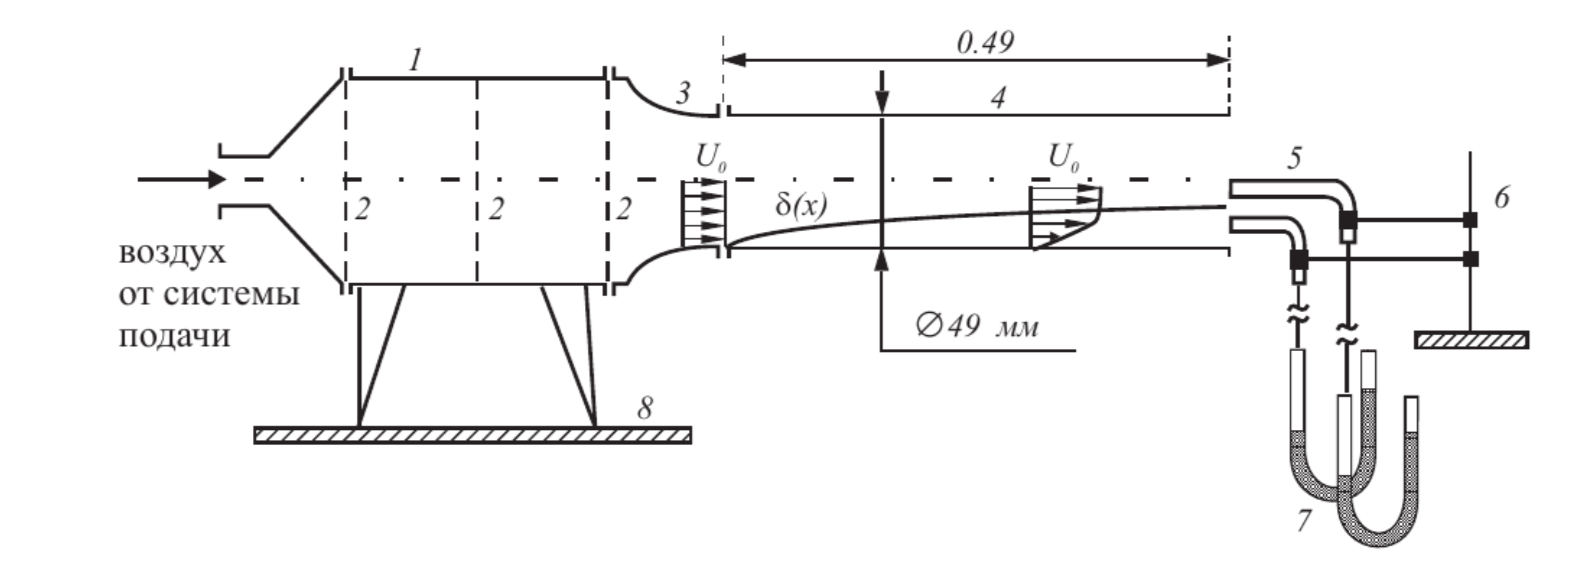
\includegraphics[width=0.9\textwidth]{mss.png} % замените на актуальное имя файла
\caption{Схема установки и системы измерений}
\end{figure}

Поток воздуха поступает в цилиндрический рабочий канал, на внутренней поверхности которого формируется пограничный слой. Толщина пограничного слоя мала по сравнению с радиусом канала, поэтому характеристики течения близки к пограничному слою на плоской пластине. Измерение параметров пограничного слоя проводится с помощью трубок полного напора, соединенных с манометрами. Трубки закреплены на координатном механизме, позволяющем перемещать их в радиальном направлении и измерять распределение скорости в сечении канала.

В процессе опыта изменялось напряжение на установке, что приводило к изменению скорости потока. Для каждого режима измерялись скоростной напор в ядре потока $\Delta P_\text{я}$, скоростной напор в фиксированной точке пограничного слоя $\Delta P_{\text{п.с.}}$, а также профиль скорости $U(y)$ для двух режимов течения.

Так как скорость потока, создаваемая установкой, менее 20 м/с, что гораздо меньше скорости звука в воздухе при комнатной температуре. Тогда формулу для сжатия идеального газа можно разложить до первого порядка:

\begin{equation}
    \frac{P_0}{P}=(1+\frac{\gamma-1}{2}M^2)^{\frac{\gamma}{\gamma-1}}\approx1+\frac{\gamma}{2}M^2=1+\frac{\gamma u^2}{2a^2}=1+\frac{\rho u^2}{2P}.
\end{equation}

Умножая на P, получим

\begin{equation}
    P_0=P+\frac{\rho u^2}{2},
\end{equation}

где $P_0$ - давление торможения, $P$ - давление статическое.

В силу малости скорости (дозвуковой поток) статическое давление на выходе установки совпадает с атмосферным давлением в комнате, поэтому для вычисления скорости можно использовать упрощенную формулу, так как прибор показывает разность давления торможения и внешней среды:

\begin{equation}
    u=\sqrt{\frac{2}{\rho}}\cdot\sqrt{\Delta P},
\end{equation}
где $\Delta P$ - измеренное на приборе значение. Для простоты расчетов введем коэффициент $k_1=\sqrt{\frac{2}{\rho}}$.

Осталось только определиться с характерным размером задачи. В силу того, что толщина турбулентного/ламинарного слоя мала, то можно рассматривать малый слой воздуха рядом с поверхностью трубы, а значит не обращать внимание на её поперечный размер. Так как исследуемый поток от создания до точки фиксации на всем пути взаимодействует с поверхности трубы, то за характерную длину мы берем  длину самой трубы. 

\section{ Проведение эксперимента и обработка результатов}
Исходя из данных о параметрах среды во время проведения эксперимента $P_{атм}=10^5 $Па и $T=295K$.

Используя формулу идеального газа $\rho=\frac{P}{RT}$, определяем $\rho=1.18$ кг/м$^3$ и $k_1=1.3$. Аналогично рассчитываем коэффициент для получения числа Рейнольдца $k_2=0.405\cdot10^5$, где $Re=k_2\sqrt{\Delta P}$.

По результатам измерений были получены следующие данные:

\begin{table}[H]
    \centering
    \caption{Зависимость параметров от напряжения}
    \label{tab:voltage_dep}
    \resizebox{\textwidth}{!}{%
    \begin{tabular}{|c|c|c|c|c|c|c|c|}
        \hline
        $U$, В & $\Delta P_{\text{п.с.}}$, Па & $\Delta P_{\text{я}}$, Па & $V_{\text{п.с.}}$, м/с & $V_{\text{я}}$, м/с & $\frac{\Delta P_{\text{п.с.}}}{\Delta P_{\text{я}}}$ & $\frac{V_{\text{п.с.}}}{V_{\text{я}}}$ & $Re \times 10^{-5}$ \\
        \hline
        80  & 31  & 38  & 7.24 & 8.01  & 0.82 & 0.90 & 2.466 \\ \hline
        90  & 36  & 44  & 7.80 & 8.62  & 0.82 & 0.90 & 2.653 \\ \hline
        100 & 44  & 52  & 8.62 & 9.37  & 0.85 & 0.92 & 2.884 \\ \hline
        110 & 48  & 60  & 9.01 & 10.07 & 0.80 & 0.89 & 3.098 \\ \hline
        120 & 50  & 68  & 9.19 & 10.72 & 0.74 & 0.86 & 3.298 \\ \hline
        130 & 49  & 77  & 9.10 & 11.41 & 0.64 & 0.80 & 3.510 \\ \hline
        140 & 49  & 85  & 9.10 & 11.99 & 0.58 & 0.76 & 3.688 \\ \hline
        150 & 52  & 93  & 9.37 & 12.54 & 0.56 & 0.75 & 3.857 \\ \hline
        160 & 55  & 102 & 9.64 & 13.13 & 0.54 & 0.73 & 4.040 \\ \hline
        180 & 63  & 117 & 10.32 & 14.06 & 0.54 & 0.73 & 4.327 \\ \hline
        200 & 72  & 133 & 11.03 & 14.99 & 0.54 & 0.74 & 4.613 \\ \hline
        220 & 80  & 147 & 11.63 & 15.76 & 0.54 & 0.74 & 4.850 \\ \hline
        240 & 88  & 162 & 12.20 & 16.55 & 0.54 & 0.74 & 5.091 \\ \hline
    \end{tabular}
    }
\end{table}

\newpage


\begin{table}[H]
    \centering
    \caption{Профиль скорости пограничного слоя (ламинарный режим, $U = 100$ В)}
    \label{tab:laminar}
    \begin{tabular}{|c|c|c|c|} % <-- Вертикальные линии
        \hline
        $y$, мм & $\Delta P_{\text{п.с.}}$, Па & $V_{\text{п.с.}}$, м/с & $V_{\text{п.с.}} / V_{\text{я}}$ \\
        \hline
        0.25 & 3   & 2.25 & 0.24 \\ \hline
        0.50 & 10  & 4.11 & 0.44 \\ \hline
        0.75 & 18  & 5.52 & 0.59 \\ \hline
        1.00 & 26  & 6.63 & 0.71 \\ \hline
        1.25 & 30  & 7.12 & 0.76 \\ \hline
        1.50 & 38  & 8.01 & 0.85 \\ \hline
        2.00 & 46  & 8.82 & 0.94 \\ \hline
        2.50 & 49  & 9.10 & 0.97 \\ \hline
        3.25 & 50  & 9.19 & 0.98 \\ \hline
        4.00 & 50  & 9.19 & 0.98 \\ \hline
        4.75 & 50  & 9.19 & 0.98 \\ \hline
    \end{tabular}
\end{table}


\begin{table}[H]
    \centering
    \caption{Профиль скорости пограничного слоя (турбулентный режим, $U = 230$ В)}
    \label{tab:turbulent}
    \begin{tabular}{|c|c|c|c|}
        \hline
        $y$, мм & $\Delta P_{\text{п.с.}}$, Па & $V_{\text{п.с.}}$, м/с & $V_{\text{п.с.}} / V_{\text{я}}$ \\
        \hline
        0.25  & 15   & 5.03  & 0.32 \\ \hline
        0.50  & 40   & 8.22  & 0.52 \\ \hline
        0.75  & 53   & 9.46  & 0.59 \\ \hline
        1.00  & 62   & 10.24 & 0.64 \\ \hline
        1.25  & 69   & 10.80 & 0.68 \\ \hline
        1.50  & 73   & 11.11 & 0.70 \\ \hline
        2.00  & 80   & 11.63 & 0.73 \\ \hline
        2.50  & 86   & 12.06 & 0.76 \\ \hline
        3.25  & 95   & 12.67 & 0.80 \\ \hline
        4.00  & 102  & 34.44 & 2.16 \\ \hline
        4.75  & 110  & 13.63 & 0.86 \\ \hline
        5.75  & 120  & 14.24 & 0.89 \\ \hline
        6.75  & 129  & 14.77 & 0.93 \\ \hline
        8.00  & 138  & 15.27 & 0.96 \\ \hline
        9.50  & 142  & 15.49 & 0.97 \\ \hline
        11.00 & 146  & 15.71 & 0.99 \\ \hline
        13.00 & 148  & 15.82 & 0.99 \\ \hline
        15.00 & 150  & 15.92 & 1.00 \\ \hline
        17.00 & 150  & 15.92 & 1.00 \\ \hline
        19.00 & 150  & 15.92 & 1.00 \\ \hline
    \end{tabular}
\end{table}

Представим в виде графиков.

\begin{figure}[H]
\centering
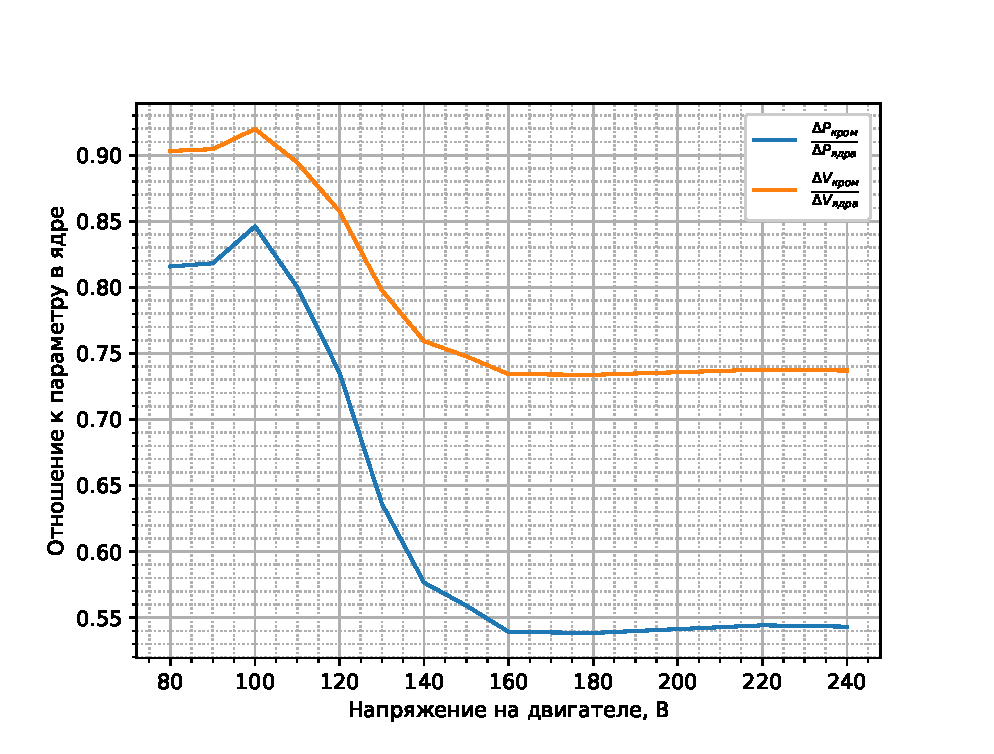
\includegraphics[width=0.9\textwidth]{FlowPar_V.eps}
\caption{Зависимость отношения скорости в ядре к скорости в пограничном слое от напряжения}
\end{figure}
\begin{figure}[H]
\centering
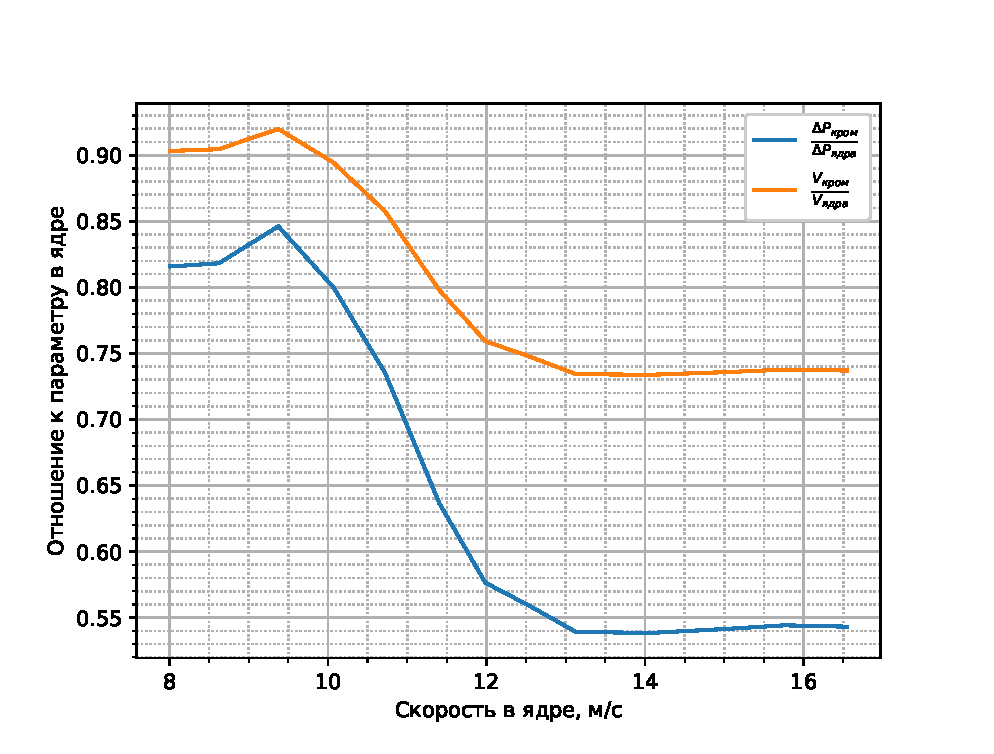
\includegraphics[width=0.9\textwidth]{FlowPar_U.eps}
\caption{Зависимость отношения скорости в ядре к скорости в пограничном слое от скорости в ядре}
\end{figure}

По графиком можно заметить, что критическая область, где ламинарный пограничный слой переходит в турбулентный при данной длине трубы начинается со скорости потока в ядре, равной $\approx9.4$ м/с.

\begin{figure}[H]
\centering
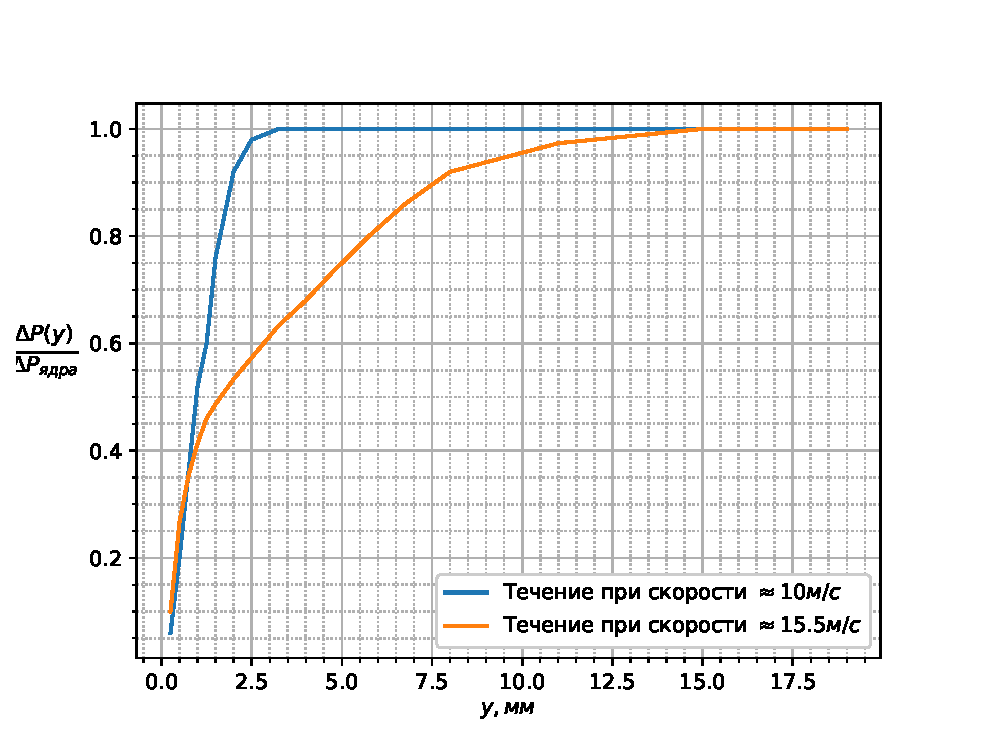
\includegraphics[width=0.9\textwidth]{PfP.eps}
\caption{Зависимость отношения давления в сечении к давлению в ядре от высоты}
\end{figure}
\begin{figure}[H]
\centering
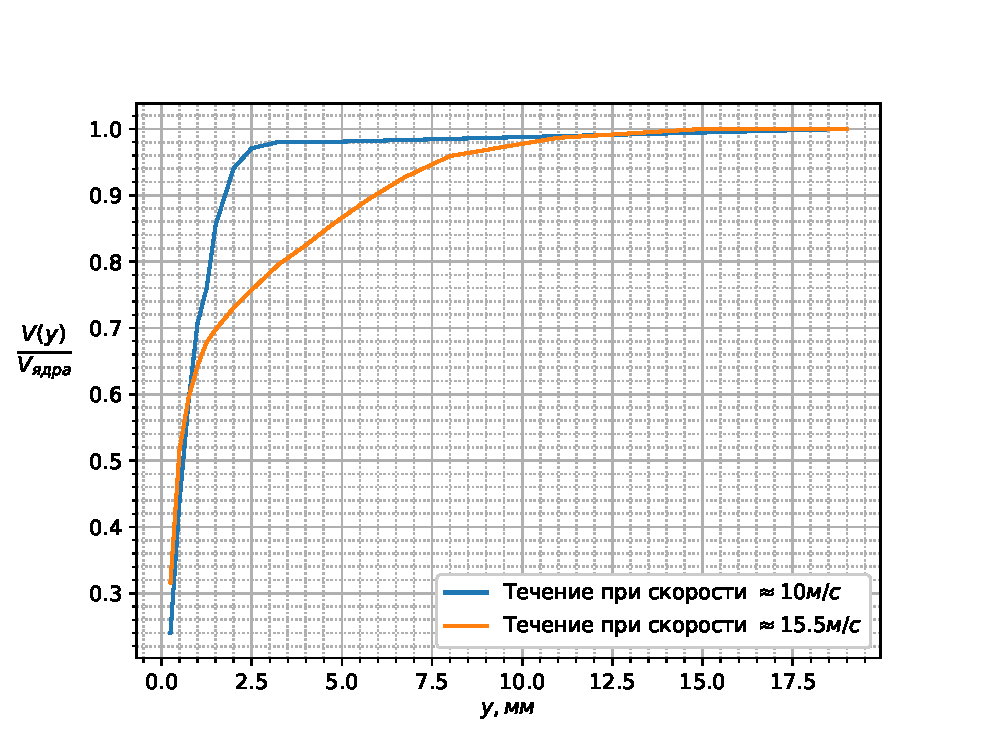
\includegraphics[width=0.9\textwidth]{VfV.eps}
\caption{Зависимость отношения скорости в сечении к скорости в ядре от высоты}
\end{figure}

По данным графикам можно качественно понять, что толщина вытеснения в случае ламинарного течения (10м/с) намного меньше, чем для турбулентного. Примерные величины $\delta^{*}_{л}=0.72$мм и $\delta^{*}_{т}=1.80$мм

\section{ Обсуждение результатов и выводы}

В ходе выполнения лабораторной работы №5 был экспериментально исследован переход ламинарного пограничного слоя в турбулентный на внутренней поверхности цилиндрического канала.

По результатам измерений установлено, что при увеличении скорости потока отношение скоростей $V_{\text{п.с.}}/V_{\text{я}}$ вначале растёт, а затем, достигнув максимума, начинает заметно уменьшаться. Этот максимум соответствует началу перехода пограничного слоя в турбулентное состояние. Для использованной в работе трубки переход начинается при скорости потока в ядре около $9.4$ м/с, что соответствует критическому числу Рейнольдса 
$$
Re_{x,кр} \approx 2.9 \times 10^5.
$$

Полученное значение лежит в типичном для аэродинамических экспериментов диапазоне ($2 \times 10^5 - 5 \times 10^5$), что подтверждает корректность проведённых измерений. Относительно низкое значение $Re_{x,кр}$ объясняется наличием остаточной турбулентности на входе в рабочий канал и возможной шероховатостью стенок.

Сравнение профилей скорости в ламинарном и турбулентном режимах показало ожидаемые различия: турбулентный профиль является более «полным», а толщина пограничного слоя и толщина вытеснения $\delta^*$ значительно больше, чем в ламинарном случае. Так, при скорости около 10 м/с $\delta^*_\text{л} \approx 0.72$ мм, а при турбулентном режиме $\delta^*_\text{т} \approx 1.80$ мм.

Переход ламинарного пограничного слоя в турбулентный на внутренней поверхности канала происходит при $Re_{x,кр} \approx 2.9 \times 10^5$.\\
При переходе наблюдается резкое увеличение толщины пограничного слоя и толщины вытеснения.\\
Турбулентный пограничный слой характеризуется более полным профилем скорости по сравнению с ламинарным.\\
Экспериментальные результаты качественно и количественно согласуются с теоретическими  о развитии пограничного слоя.
\end{document}
